La morphologie mathématique a, en 1964, d'abord été introduite sous sa forme binaire \cite{Serra_1986}. Dans ce cadre, les images peuvent être définies soit de manière ensembliste, où elles et les objets contenus en elles sont définis comme des parties d'un ensemble E structuré comme un groupe pour l'addition, soit, par équivalence, de manière fonctionnelle booléenne, où les images sont définies comme fonctions sur un sous-ensemble de $E$ à valeurs dans $\{0,1\}$, où $1$ est associé aux objets et $0$ au fond de l'ensemble de définition \cite{Serra_1983}. Dans un contexte discret, tel que les images, on a $E=\mathbb{Z}^2$. \\

\vspace{-1.6mm}
Les opérations fondamentales de la morphologie mathématique sont l'érosion et la dilatation. Dans le cadre binaire, elles sont définies de manière ensembliste sur $E$. \\

\vspace{-1.6mm}
\noindent Soit $B \subset E$ l'élément structurant, servant de structure aux opérations morphologiques.

\noindent On définit $B_x$ comme l'ensemble $B$ translaté de $x \in E$ : \hspace{0.444cm} $B_x = \{ \, b+x \, \mid \, b \in B \, \}$

\noindent On définit $\breve{B}$ \hspace{0.7mm} comme l'ensemble symétrique de $B$ : \hspace{1.03cm} $\breve{B}$ \hspace{0.02mm} $= \{ \, -b \, \mid \, b \in B \, \}$

\vspace{0.4cm}
\begin{itemize}[leftmargin=*]
    \item[$\bullet$] L'érosion $\epsilon_B(X)$ d'une partie $X$ de $E$ par l'élément structurant $B$ est définie par : 
    \begin{equation}
        \epsilon_B(X) = X \ominus B = \{ \, x \, \mid \, B_x \subset X \, \}
        \label{binary_erosion}
    \end{equation}
\end{itemize}
\vspace{0cm}
\begin{itemize}[leftmargin=*]
    \item[$\bullet$] La dilatation $\delta_B(X)$ de $X$ par $B$ est, quant à elle, définie par : 
    \begin{equation}
        \delta_B(X) = X \oplus B = \{ \, x \, \mid \, \breve{B}_x \cap X \neq \emptyset \, \}
        \label{binary_dilation}
    \end{equation}
\end{itemize}

%figure
\vspace{-1.5mm}
\begin{figure}[ht]
  \begin{center}
      \subfigure[Image originale]{
          
\includegraphics[width=0.28\textwidth]{parts/2-etat_de_lart/A-operateurs_morphologiques_classiques/figures/BI_original.png}
          \label{fig:sub1}}\hfill
      \subfigure[Image érodée]{
          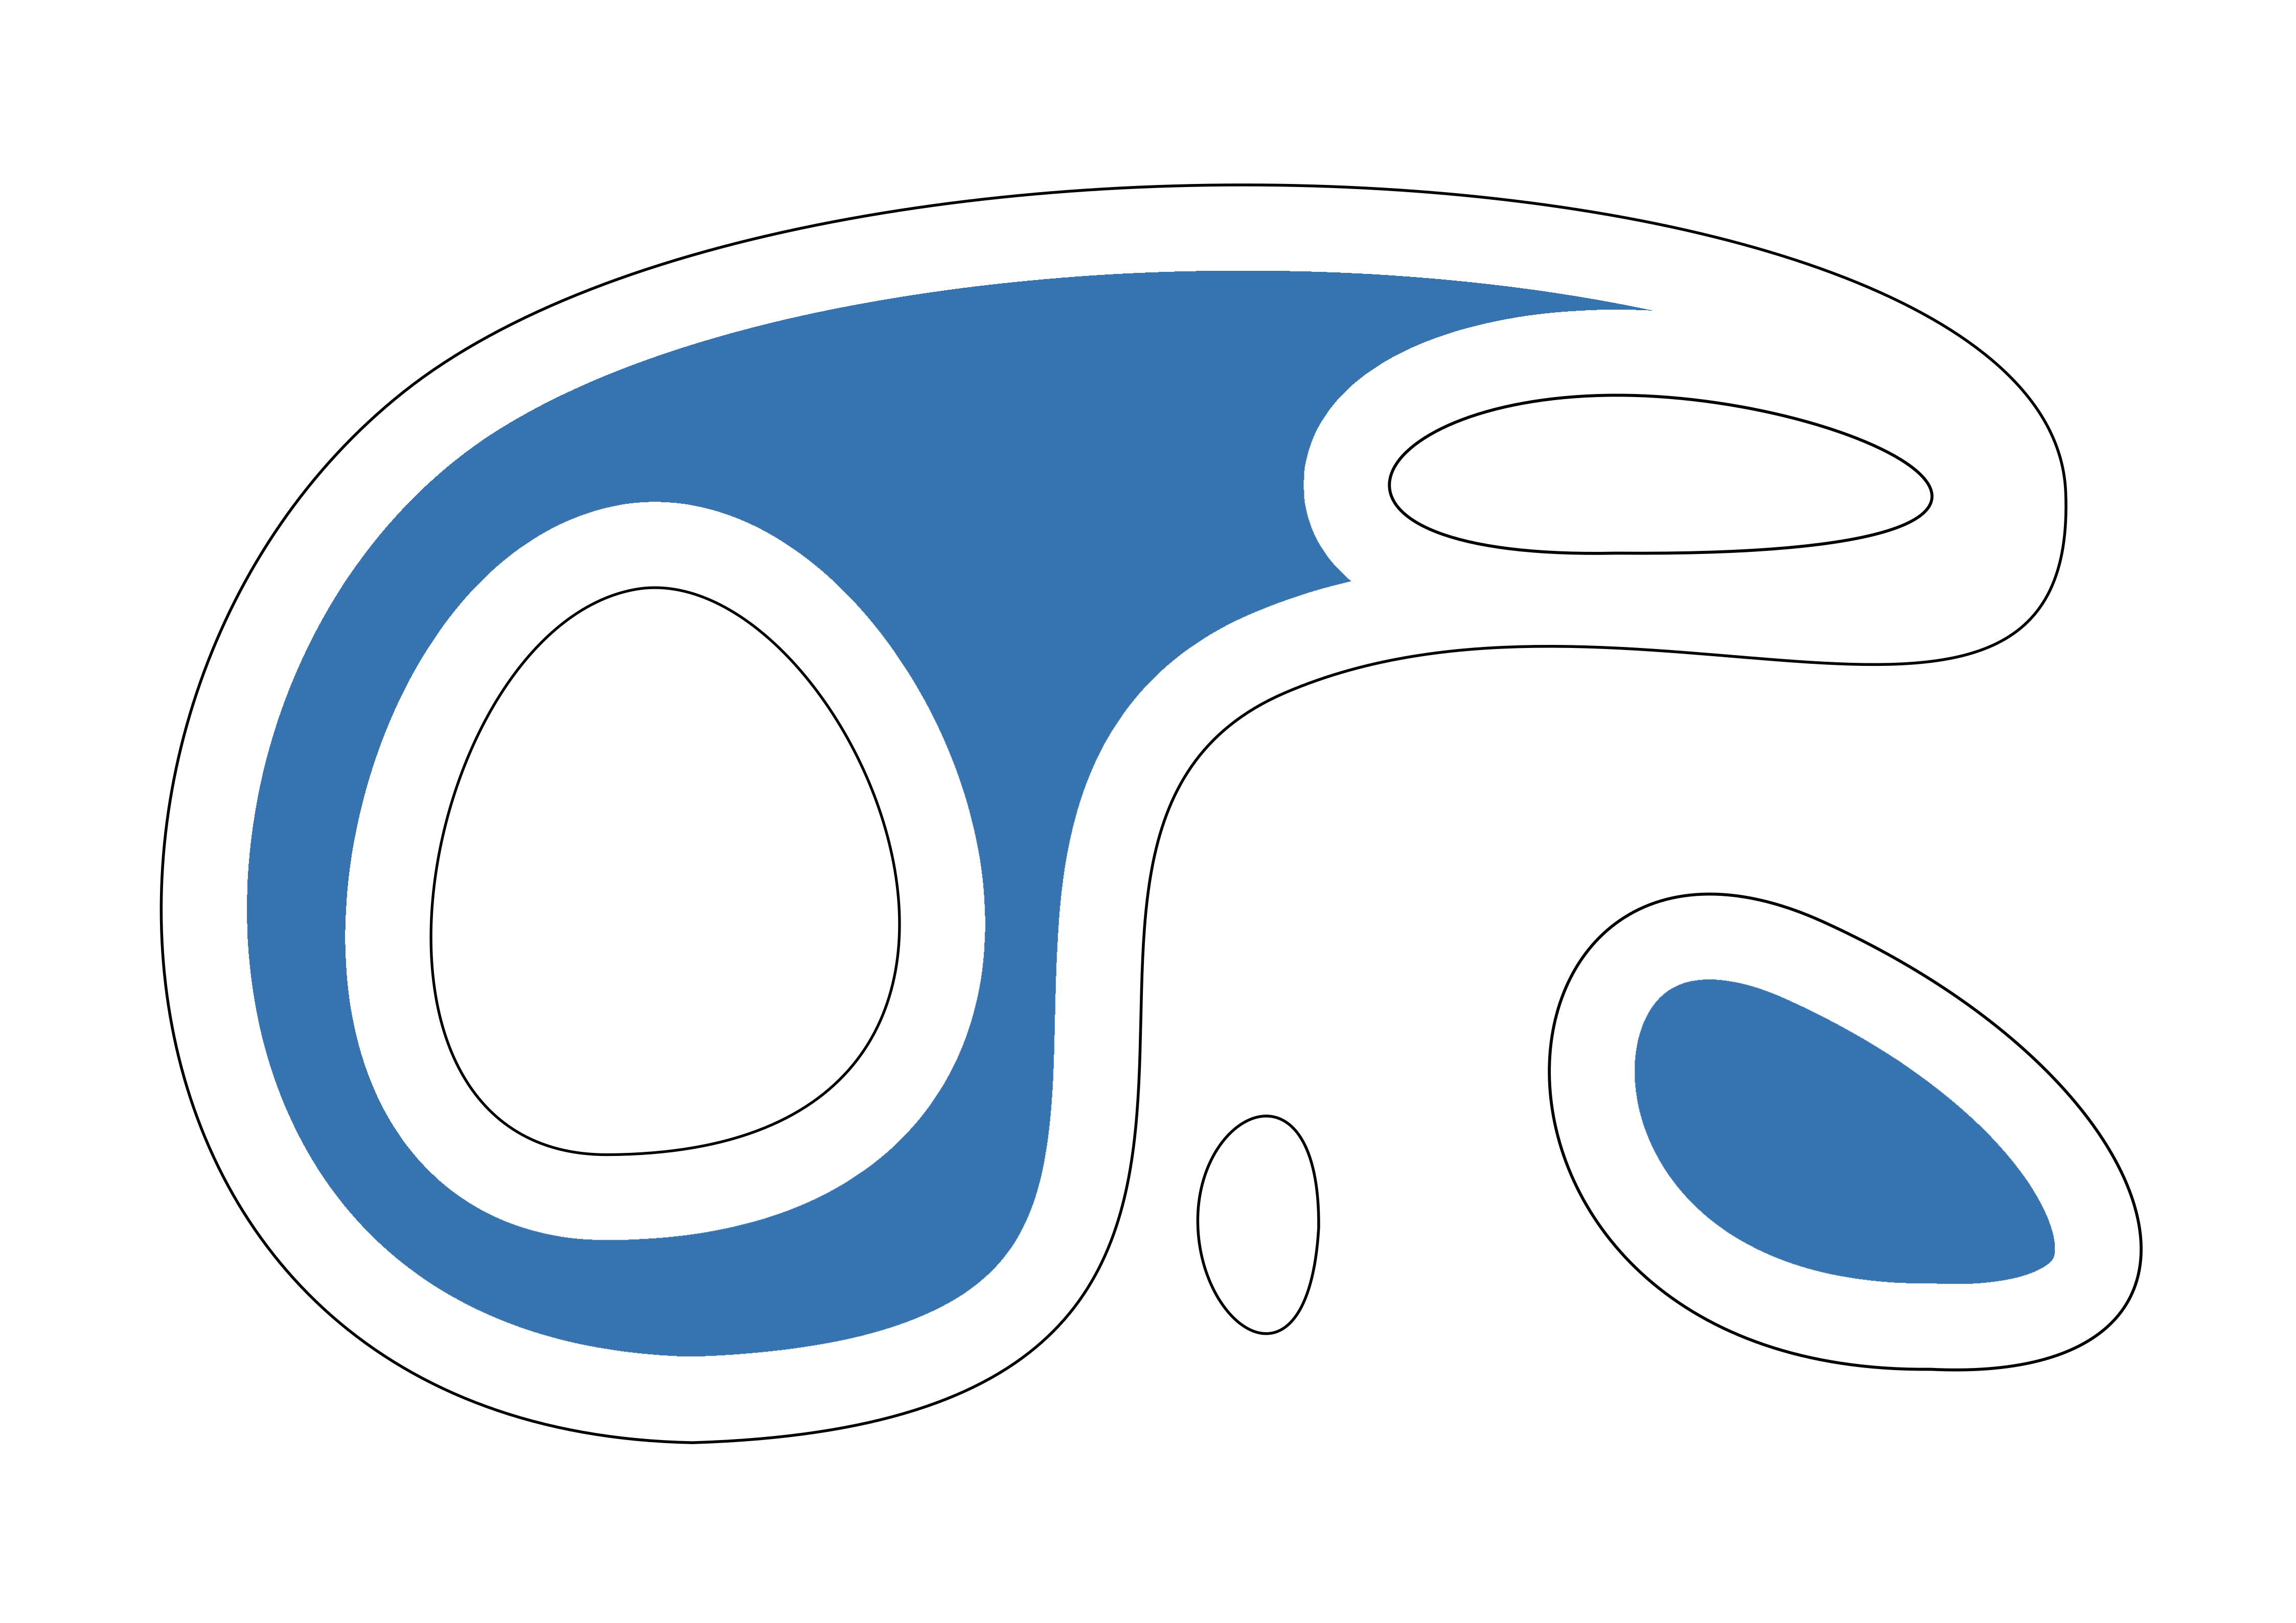
\includegraphics[width=0.28\linewidth]{parts/2-etat_de_lart/A-operateurs_morphologiques_classiques/figures/BI_eroded.png}
          \label{fig:sub2}}\hfill
      \subfigure[Image dilatée]{
          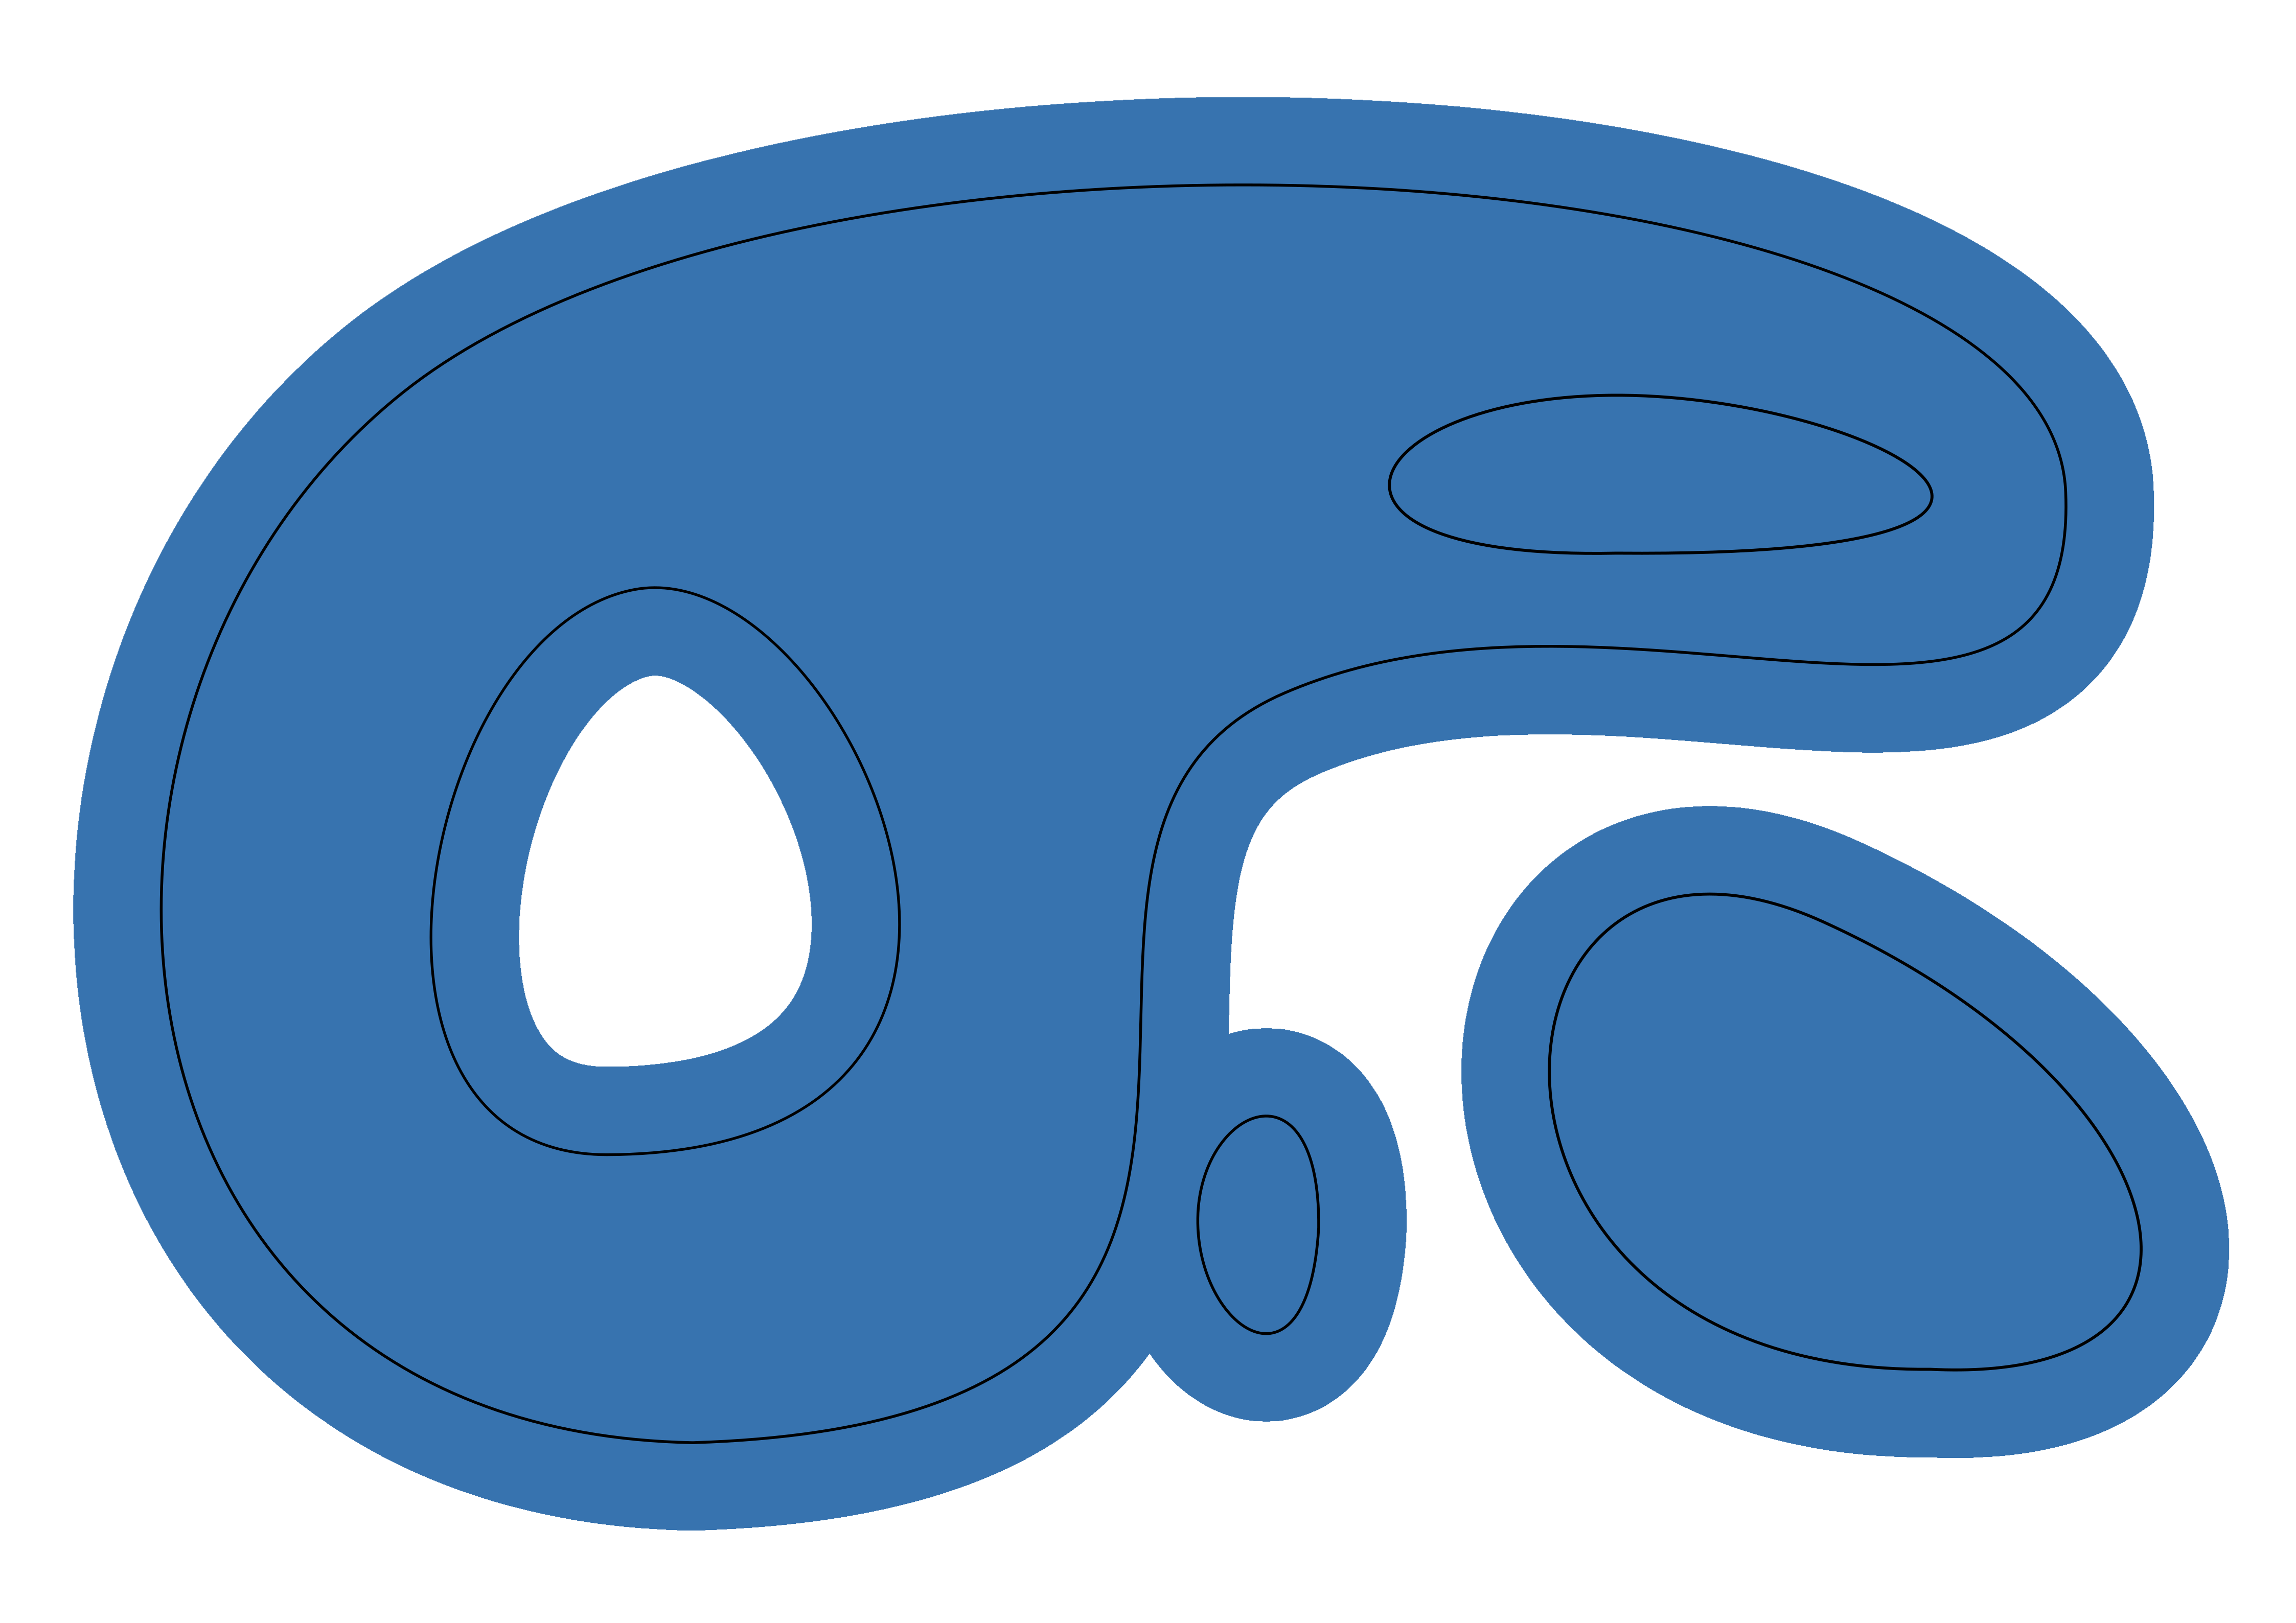
\includegraphics[width=0.28\textwidth]{parts/2-etat_de_lart/A-operateurs_morphologiques_classiques/figures/BI_dilated.png}
          \label{fig:sub3}}\hfill
      \subfigure[B]{
          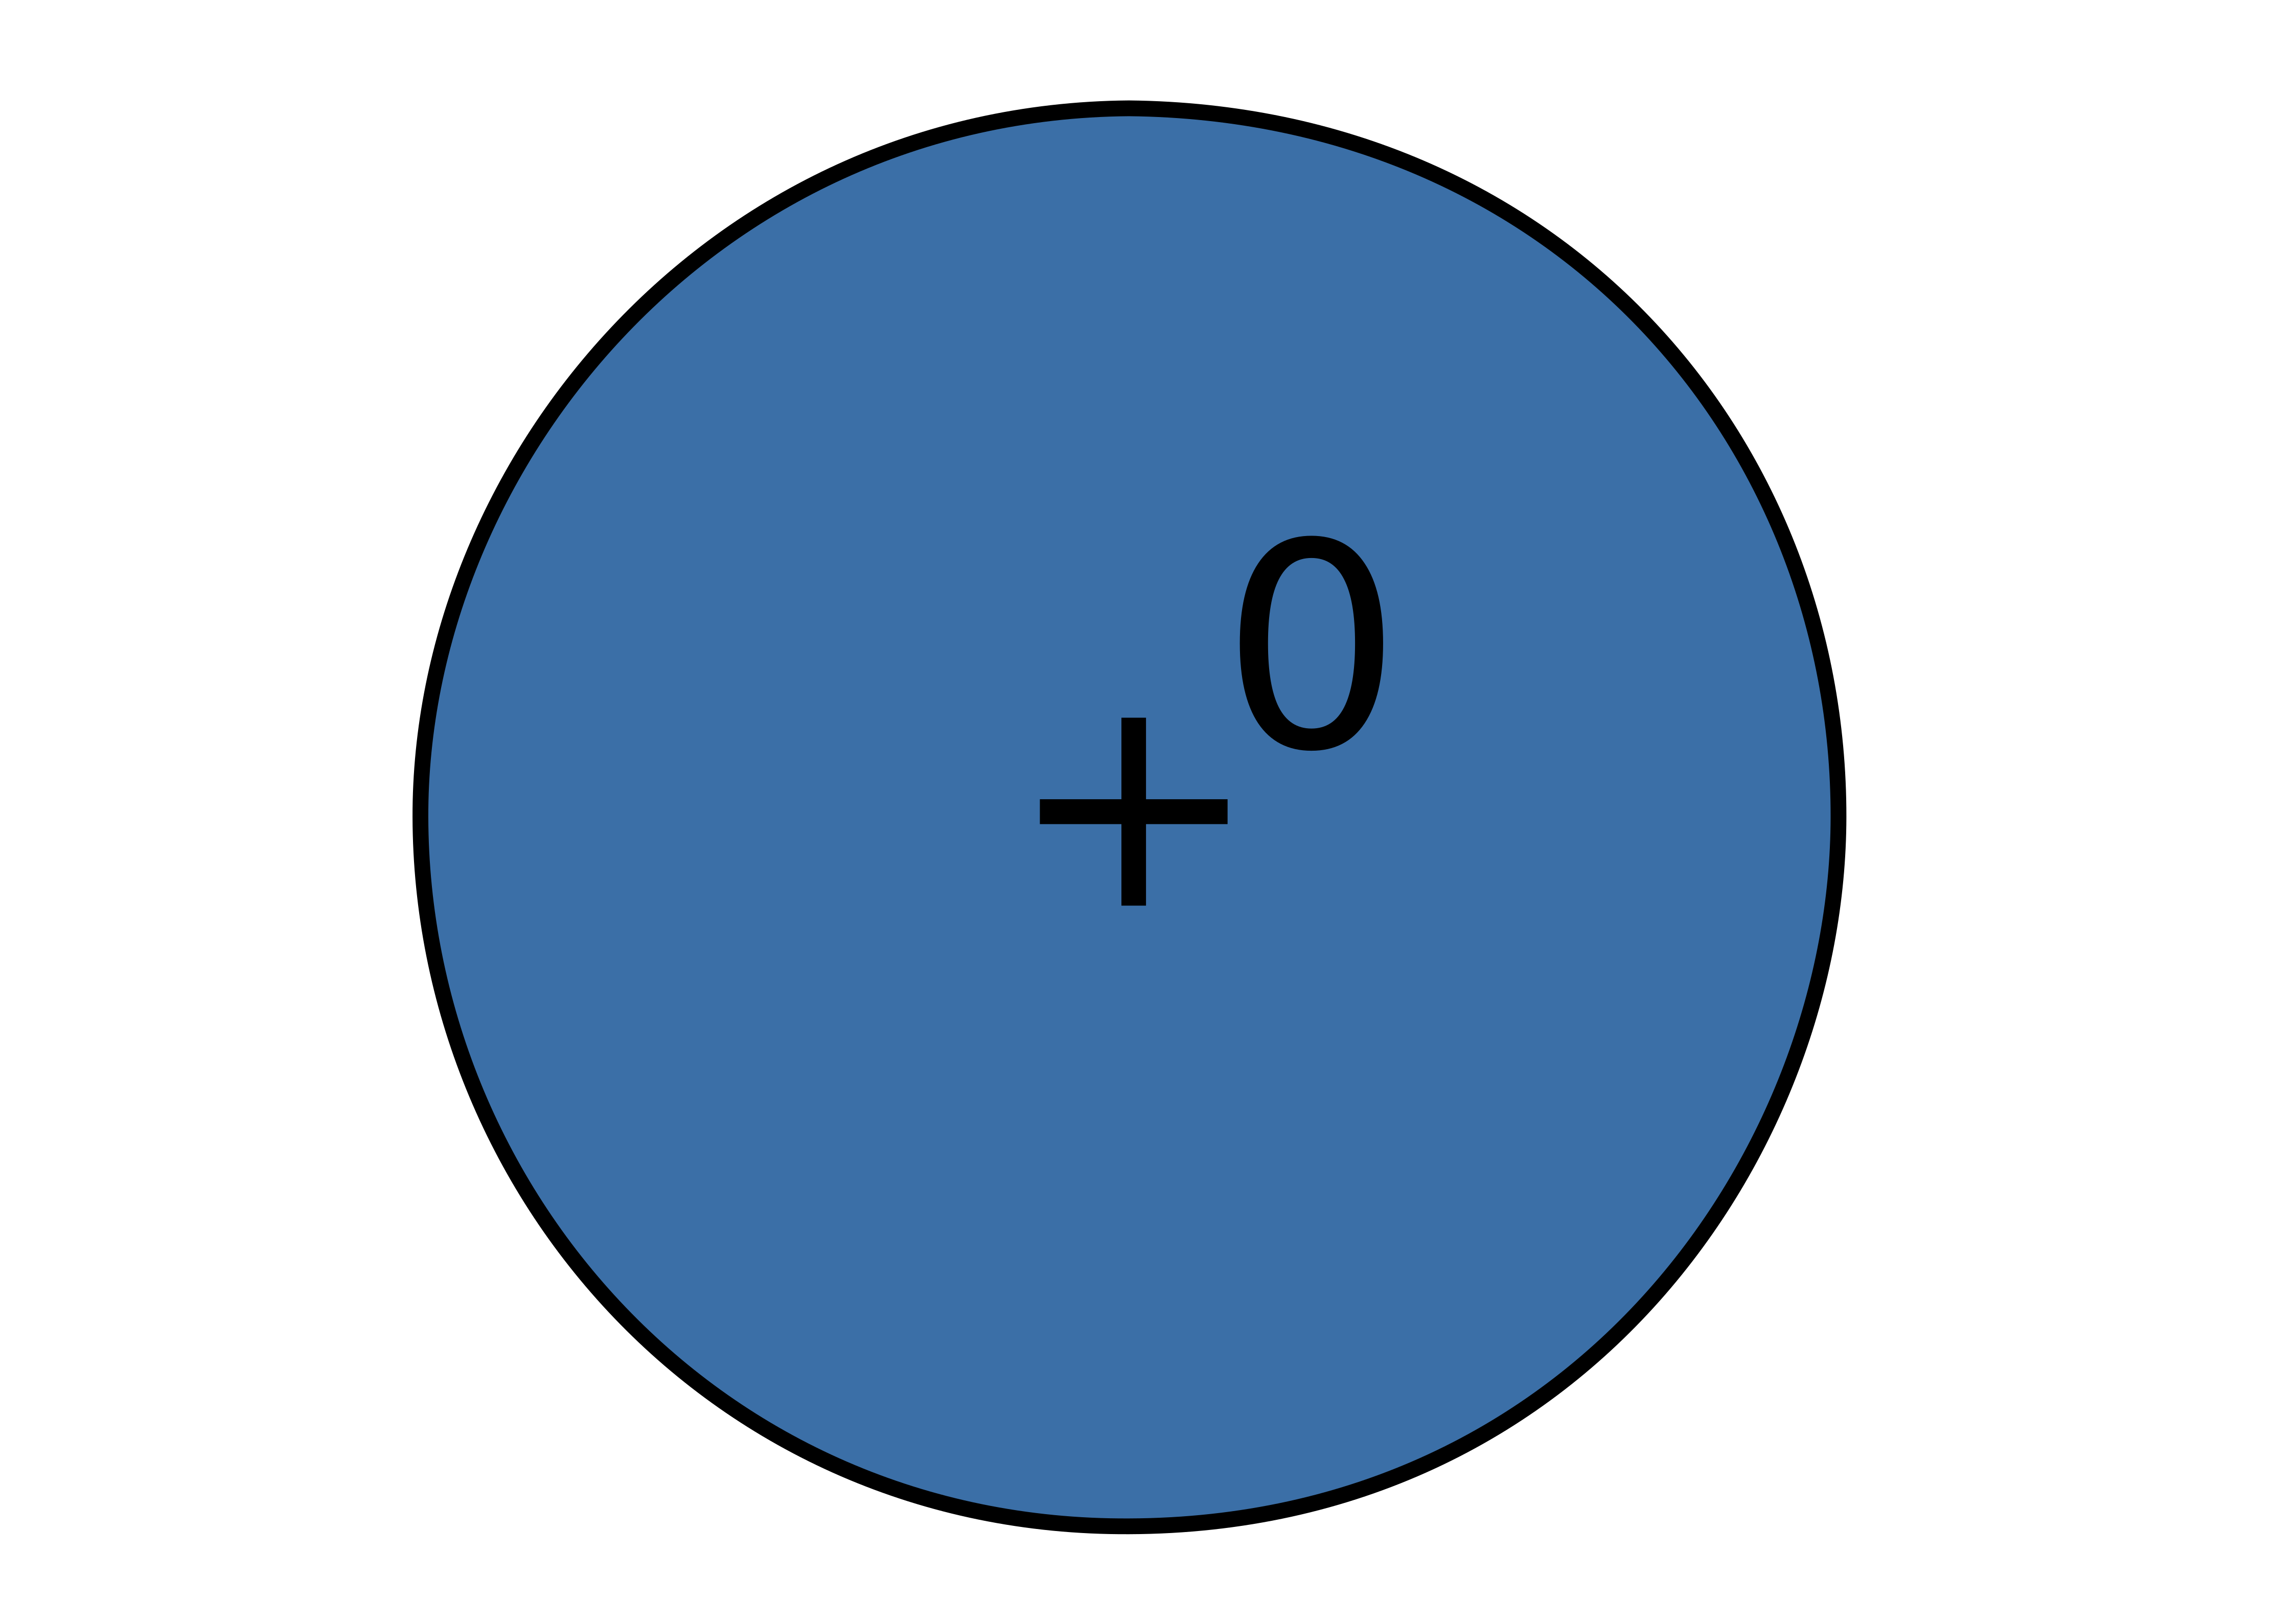
\includegraphics[width=0.05\textwidth]{parts/2-etat_de_lart/A-operateurs_morphologiques_classiques/figures/BI_selem.png}
          \label{fig:sub4}}
    \caption{ \centering Exemple de l'érosion $\ominus$ \ref{fig:sub2} et de la dilatation $\oplus$ \ref{fig:sub3} d'une image binaire \ref{fig:sub1} par un élément structurant binaire $B$ en forme de disque centré en $(0,0)$, fig. \ref{fig:sub4}.}
    \label{fig:morpho_binary_operations_example}
  \end{center}
\end{figure}

\vspace{-1.6mm}
En combinant l'érosion (\ref{binary_erosion}) et la dilatation (\ref{binary_dilation}), illustrées fig. \ref{fig:morpho_binary_operations_example}, on peut créer des opérations plus avancées, telles l'ouverture $\circ$ : $\gamma_B(X) = \delta_B(\epsilon_B(X))$ ; la fermeture $\bullet$ : $\phi_B(X) = \epsilon_B(\delta_B(X))$ ; ou encore le gradient morphologique : $\text{grad}_B(X)=\delta_B(X)-\epsilon_B(X)$.

\vfill

%%% ASPECT ENSEMBLISTE (on considère des sous-ensembles de Z²)